\documentclass[11pt, oneside]{article}
\usepackage[letterpaper, margin=2cm]{geometry}
\usepackage{MATH566}
%\usepackage{sagetex}

\begin{document}
\noindent \textbf{\Large{Caleb Logemann \\
MATH 566 Discrete Optimization\\
Homework 5
}}

%\lstinputlisting[language=Sage]{03_2.sage}
\begin{enumerate}
  \item % #1 Done
    Let $S$ be defined as intersection of halfspaces $x_i \geq 0$ and $(1-x_i)^k \geq 0$.
    Suppose $i \in \{1,2,\ldots,d\}$ and $k \geq 1$ is odd.
    Compute the analytic center of $S$.
    Notice that for $x$ satisfying $(1-x_i)^k \geq 0$, the function $(1-x_i)^k$ is convex.

    Each of the halfspaces can be rewritten as $-(1 - x_i)^k \le 0$ and
    $-x_i \le 0$, therefore the logarithmic barrier function for this set is
    \[
      \Phi(\v{x}) = -\sum{i = 1}{d}{\ln{(1 - x_i)^k}} - \sum{i=1}{d}{\ln{x_i}}
    \]
    This can be simplified to
    \[
      \Phi(\v{x}) = -k\sum{i = 1}{d}{\ln{1 - x_i}} - \sum{i=1}{d}{\ln{x_i}}
    \]

    Now the analytic center of $S$ is the value $\v{x}^*$ which minimizes $\Phi(\v{x})$.
    This value can be found using calculus, by finding the value of each $x_i$
    that makes $\pd{\Phi}{x_i} = 0$ respectively.
    \begin{align*}
      \pd{\Phi}{x_i} = -k\frac{1}{x_i - 1} - \frac{1}{x_i} \\
      0 &= -k\frac{1}{x_i - 1} - \frac{1}{x_i} \\
      0 &= \frac{-k x_i - x_1 + 1}{x_i(x_i - 1)} \\
      0 &= -(k+1)x_i + 1 \\
      x_i &= \frac{1}{k+1} \\
    \end{align*}
    This is true for any $x_i$ with $1 \le i \le d$.
    Also since $(1 - x_i)^k$ is convex function we know that this critical point
    is a minima.
    Therefore the analytic center of $S$ is
    $\p{\frac{1}{k+1}, \cdots, \frac{1}{k+1}} \in \RR^d$.

  \item % #2 Done 
    Compute central path for the following problem
    \[
      (P)
      \begin{cases} 
        \text{minimize }   & -x_1 \\
        \text{subject to } & x_1 \leq 1 \\
                           & x_2 \leq 1 \\
                           & x_1 \geq 0 \\
                           & x_2 \geq 0
      \end{cases}
    \]
    and find the optimal solution using the central path.
    Plot (sketch) the set of feasible solutions and the computed central path.
    Lot of calculus...

    The constraints can be rewritten as
    \[
      (P)
      \begin{cases} 
        \text{minimize }   & -x_1 \\
        \text{subject to } & x_1 - 1 \leq 0 \\
                           & x_2 - 1 \leq 0 \\
                           & -x_1 \leq 0 \\
                           & -x_2 \leq 0
      \end{cases}
    \]
    The logarithmic barrier function for this linear program
    \[
      \Phi(\v{x}) = -\ln{1 - x_1} - \ln{1 - x_2} - \ln{x_1} - \ln{x_2}
    \]
    The central path can be found minimizing
    \[
      P_t(x_1, x_2) = t (-x_1) + -\ln{1 - x_1} - \ln{1 - x_2} - \ln{x_1} - \ln{x_2}
    \]
    with respect to $x_1$ and $x_2$.
    In order to do this we need to take the partial derivatives of $P_t$ with
    respect to $x_1$ and $x_2$.
    \begin{align*}
      \pd{P_t}{x_1} = -t + \frac{1}{1 - x_1} - \frac{1}{x_1} \\
      \pd{P_t}{x_2} = \frac{1}{1 - x_2} - \frac{1}{x_2}
    \end{align*}
    Now setting these derivatives equal to zero we can find a parametrized
    function for the central path.
    \begin{align*}
      \pd{P_t}{x_2} &= 0 \\
      0 &= \frac{1}{1 - x_2} - \frac{1}{x_2} \\
      0 &= \frac{x_2 - 1 + x_2}{(1 - x_2)x_2} \\
      0 &= 2x_2 - 1 \\
      x_2 &= \frac{1}{2} \\
      \pd{P_t}{x_1} &= 0 \\
      0 &= -t + \frac{1}{1 - x_1} - \frac{1}{x_1} \\
      0 &= \frac{-t(1 - x_1)x_1 + x_1 - 1 + x_1}{(1 - x_1)x_1} \\
      0 &= -t x_1^2 + (2 - t)x_2 - 1 \\
      x_1 &= \frac{t - 2 \pm \sqrt{(2-t)^2 + 4t}}{2t} \\
      x_1 &= \frac{1}{2} - \frac{1}{t} \pm \sqrt{\frac{1}{t^2} + \frac{1}{4}} \\
    \end{align*}
    For $t \ge 0$, only one of the solution is in the feasible region.
    Thus the central path is
    \[
      \p{\frac{1}{2} - \frac{1}{t} \pm \sqrt{\frac{1}{t^2} + \frac{1}{4}}, \frac{1}{2}}
    \]
    for $t \ge 0$.
    This central path starts at $\p{\frac{1}{2}, \frac{1}{2}}$ and approaches
    $\p{1, \frac{1}{2}}$ as $t \to \infty$.

    A plot of the feasible region and central path is shown below.
    \begin{center}
      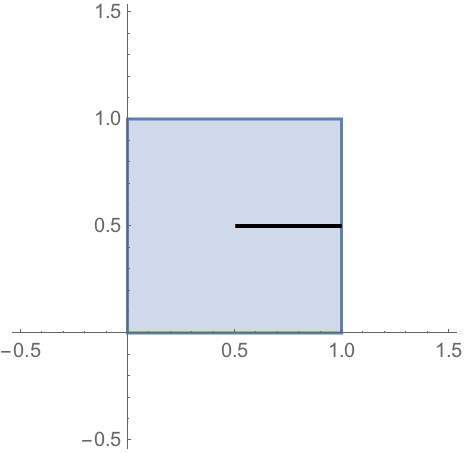
\includegraphics[scale=.5]{Figures/05_1.png}
    \end{center}

  \item % #3 Done
    Let $G=(V,E)$ and $|V|=n$.

    Recall that the spanning tree polytope was created by constraints \emph{tree has $n-1$ edges}
    and \emph{tree has no cycles}. Formally,
    \[
      STP = 
      \left\{
        \textbf{x} \in [0,1]^{E(G)}: \sum*{e \in E}{}{x_e} = n-1, \sum*{uv \in E, u\in X, v \in X}{}{x_{(u,v)}} \leq |X|-1 \text{ for } \emptyset \subset X \subset V
      \right\}.
    \]


    Suppose we try to characterize the spanning tree by assuming that by 
    constraints \emph{tree has $n-1$ edges} and \emph{tree is connected}.
    The tree is connected can be formulated by saying that for every cut, the sum $x_e$ of edges $e$ in the cut is at least one. Formally,
    \[
      P = 
      \left\{
        \textbf{x} \in [0,1]^{E(G)}: \sum*{e \in E}{}{x_e} = n-1, \sum*{uv \in E, u\in X, v \not\in X}{}{x_{(u,v)}} \geq 1 \text{ for } \emptyset \subset X \subset V
      \right\}.
    \]
    \begin{enumerate}
      \item Prove that the spanning tree polytope is a subset of $P$. That is, $STP \subseteq P$.
        \begin{proof}
          Let $x \in STP$, then $\sum{e \in E}{}{x_e} = n-1$ and
          $\sum*{uv \in E, u\in X, v \in X}{}{x_{(u,v)}} \leq |X|-1$ for every
          $\emptyset \subset X \subset V$.
          Note that
          \[
            \sum*{uv \in E, u\in X, v \in X}{}{x_{(u,v)}} +
            \sum*{uv \in E, u\in X, v \not\in X}{}{x_{(u,v)}} =
            \sum{e \in E}{}{x_e}
          \]
          Simplifying
          \[
            \sum*{uv \in E, u\in X, v \not\in X}{}{x_{(u,v)}} =
            n - 1 - \sum*{uv \in E, u\in X, v \in X}{}{x_{(u,v)}}
          \]
          Using $\sum*{uv \in E, u\in X, v \in X}{}{x_{(u,v)}} \leq |X|-1$
          \begin{align*}
            \sum*{uv \in E, u\in X, v \not\in X}{}{x_{(u,v)}} &\ge
            n - 1 - \abs{X} + 1 \\
            &\ge n - \abs{X}
            \intertext{Since $X \subset A$, $\abs{X} \le n-1$, therefore}
            \sum*{uv \in E, u\in X, v \not\in X}{}{x_{(u,v)}} &\ge 1
          \end{align*}
          Thus $x \in P$ as well, and therefore $STP \subset P$.
        \end{proof}

      \item Show $P$ does NOT have to be the same as the spanning tree polytope. To do this, show that
        the polytope $P$ does NOT have to be integral (i.e., $P$ contains a vertex that does not have all coordinates integers).

        For this problem, consider the graph with weights shown below.
        \begin{center}
          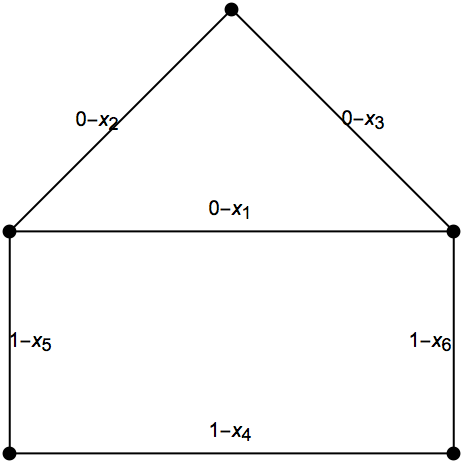
\includegraphics[scale=.5]{Figures/05_2.png}
        \end{center}

        If we minimize $\sum{i = 1}{6}{c_i x_i}$ over the polytope $P$, we will
        arrive at one of the vertices of $P$.
        Note that this linear program is essentially minimize $x_4 + x_5 + x_6$ such
        that $x_4 + x_5 \ge 1$, $x_5 + x_6 \ge 1$ and $x_4 + x_6 \ge 1$.
        The values that achieve this minimization are
        $x_4 = x_5 = x_6 = \frac{1}{2}$. and $x_1 = x_2 = 1$ and 
        Now $x_1 + x_2 + x_3 = 2.5$, so arbitrarily we can let $x_1 = x_2 = 1$
        and $x_3 = .5$, since these don't affect the objective function.
        This is a vertex of the polytope $P$, but it doesn't contain all integer
        coordinates.
        This implies that this is not a vertex of $STP$ as all vertices of $STP$
        have integer coordinates.
        Thus $STP \neq P$.
    \end{enumerate}
    % Hint: See the book Combinatorial Optimization from Korte and Vygen on the bottom of the page 150. Free PDF available from ISU library.

  \item % #4 Done
    Implement any minimum spanning tree algorithm and test it on random data.
    You can pick any algorithm you like. You can use ANY programming language but you have to IMPLEMENT the method yourself (calling a library function \texttt{RunKruskal} is not acceptable).
    Obtain data by randomly generating 10 points in range $[0,10]^2$ and the cost of every edge is the Euclidean distance in $\mathbb{R}^2$.
    We consider all 45 edges of $K_{10}$.
    Finally, create the plot of of the random points and draw edges picked to the spanning tree. You should provide: Name of the algorithm you implemented and short description of implementation, printout of the source code, pictures of two solutions.\\
    Template is provided for Sage, you do not have to use it.\\
    Time complexity DOES NOT matter. 

    I implemted Kruskal's algorithm in the following function.
    \lstinputlisting[language=Sage]{kruskal.sage}
    This function adds minimal edges as long as the edge doesn't connect
    a subtree to itself.
    The function does this by keeping track of which vertex is part of which
    subtree.

    The following script runs this function with a random $K_{10}$ graph.
    \lstinputlisting[language=Sage]{05_4.sage}
    The following two plots were generated by running this script twice.
    \begin{center}
      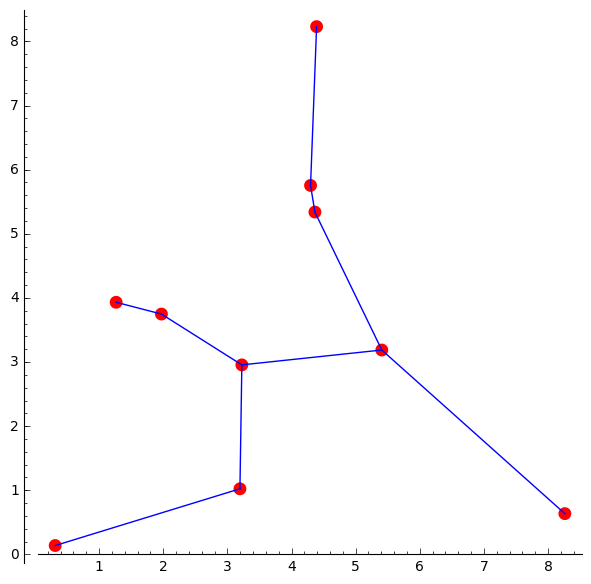
\includegraphics[scale=.5]{Figures/05_3.png} \\
      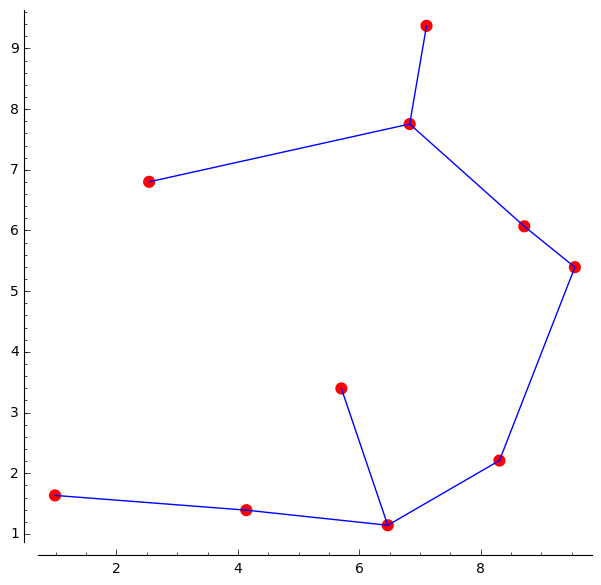
\includegraphics[scale=.5]{Figures/05_4.png}
    \end{center}
\end{enumerate}
\end{document}
